% LaTeX template for DLD Lab - runs with MikTeX and other platforms

\documentclass{article}
\usepackage{mathptmx}
\usepackage{amssymb}
\usepackage{amsfonts}
\usepackage{amsmath}
\usepackage{latexsym}
\usepackage{setspace}
\usepackage{verbatim}

\usepackage[dvipsnames]{xcolor}
\usepackage{matlab-prettifier}
\usepackage{float}
\usepackage[export]{adjustbox}



\numberwithin{equation}{section}
\newtheorem{thm}{Theorem}[section]
\newtheorem{dfn}[thm]{Definition}
\newtheorem{lem}[thm]{Lemma}
\newtheorem{rem}[thm]{Remark}
\newtheorem{cor}[thm]{Corollary}
\newtheorem{prop}[thm]{Proposition}
\newtheorem{asm}[thm]{Assumption}
\newtheorem{example}[thm]{Example}

\newenvironment{proof}{\noindent {\bf Proof.\/}}{$\qed$\vskip 0.1in}
\def\qed{ \hfill \vrule width.2cm height.2cm depth0cm\smallskip}

\usepackage{xcolor}
\usepackage{listings}
\usepackage{pythonhighlight}

\definecolor{mGreen}{rgb}{0,0.6,0}
\definecolor{mGray}{rgb}{0.5,0.5,0.5}
\definecolor{mPurple}{rgb}{0.58,0,0.82}
\definecolor{backgroundColour}{rgb}{0.95,0.95,0.92}

\lstdefinestyle{CStyle}{
    backgroundcolor=\color{backgroundColour},   
    commentstyle=\color{mGreen},
    keywordstyle=\color{magenta},
    numberstyle=\tiny\color{mGray},
    stringstyle=\color{mPurple},
    basicstyle=\footnotesize,
    breakatwhitespace=false,         
    breaklines=true,                 
    captionpos=b,                    
    keepspaces=true,                 
    numbers=left,                    
    numbersep=5pt,                  
    showspaces=false,                
    showstringspaces=false,
    showtabs=false,                  
    tabsize=2,
    language=C
}

\DeclareMathOperator*{\argmax}{argmax} % thin space, limits underneath in displays


% For minted -> Python
\usepackage{tcolorbox}
\tcbuselibrary{minted,breakable,xparse,skins}
\definecolor{bg}{gray}{0.95}
\DeclareTCBListing{mintedbox}{O{}m!O{}}{%
  breakable=true,
  listing engine=minted,
  listing only,
  minted language=#2,
  minted style=default,
  minted options={%
    linenos,
    gobble=0,
    breaklines=true,
    breakafter=,,
    fontsize=\small,
    numbersep=8pt,
    #1},
  boxsep=0pt,
  left skip=0pt,
  right skip=0pt,
  left=25pt,
  right=0pt,
  top=3pt,
  bottom=3pt,
  arc=5pt,
  leftrule=0pt,
  rightrule=0pt,
  bottomrule=2pt,
  toprule=2pt,
  colback=bg,
  colframe=orange!70,
  enhanced,
  overlay={%
    \begin{tcbclipinterior}
    \fill[orange!20!white] (frame.south west) rectangle ([xshift=20pt]frame.north west);
    \end{tcbclipinterior}},
  #3}



\numberwithin{equation}{section}
\newcommand{\cA}{\mathcal{A}}
\newcommand{\cB}{\mathcal{B}}
\newcommand{\cC}{\mathcal{C}}
\newcommand{\cD}{\mathcal{D}}
\newcommand{\cE}{\mathcal{E}}
\newcommand{\cF}{\mathcal{F}}
\newcommand{\cG}{\mathcal{G}}
\newcommand{\cH}{\mathcal{H}}
\newcommand{\cI}{\mathcal{I}}
\newcommand{\cJ}{\mathcal{J}}
\newcommand{\cK}{\mathcal{K}}
\newcommand{\cL}{\mathcal{L}}
\newcommand{\cM}{\mathcal{M}}
\newcommand{\cN}{\mathcal{N}}
\newcommand{\cO}{\mathcal{O}}
\newcommand{\cP}{\mathcal{P}}
\newcommand{\cQ}{\mathcal{Q}}
\newcommand{\cR}{\mathcal{R}}
\newcommand{\cS}{\mathcal{S}}
\newcommand{\cT}{\mathcal{T}}
\newcommand{\cU}{\mathcal{U}}
\newcommand{\cV}{\mathcal{V}}
\newcommand{\cW}{\mathcal{W}}
\newcommand{\cX}{\mathcal{X}}
\newcommand{\cY}{\mathcal{Y}}
\newcommand{\cZ}{\mathcal{Z}}
%greeks
\newcommand{\te}{{\theta}}
\newcommand{\Te}{{\Theta}}
\newcommand{\vt}{{\vartheta}}
\newcommand{\Om}{{\Omega}}
\newcommand{\om}{{\omega}}
\newcommand{\ups}{{\upsilon}}
\newcommand{\ve}{{\varepsilon}}
\newcommand{\del}{{\delta}}
\newcommand{\Del}{{\Delta}}
\newcommand{\gam}{{\gamma}}
\newcommand{\Gam}{{\Gamma}}
\newcommand{\vf}{{\varphi}}
\newcommand{\Sig}{{\Sigma}}
\newcommand{\sig}{{\sigma}}
\newcommand{\al}{{\alpha}}
\newcommand{\be}{{\beta}}
\newcommand{\ka}{{\kappa}}
\newcommand{\la}{{\lambda}}
\newcommand{\La}{{\Lambda}}


\def \D{\mathbb{D}}
\def \E{\mathbb{E}}
\def \F{\mathbb{F}}
\def \H{\mathbb{H}}
\def \L{\mathbb{L}}
\def \M{\mathbb{M}}
\def \N{\mathbb{N}}
\def \P{\mathbb{P}}
\def \Q{\mathbb{Q}}
\def \R{\mathbb{R}}
\def \Z{\mathbb{Z}}
\def \Sb{\mathbb {S}}

\def \om{\omega}
\def \Om{\Omega}
\def \ep{\epsilon}

\def\reff#1{{\rm(\ref{#1})}}

\usepackage{times}	   % uncomment to use Times-Roman fonts
%\usepackage{mathpazo}     % uncomment to use Palatino fonts
\usepackage{amsmath}	   % enable amsmath features
\usepackage{graphicx}      % enable inclusion of eps graphs
\usepackage{cite}          % bibliographical citations
\usepackage{url}           % typesetting URL's
\usepackage{color}

% ---------------------------------------------------------------

\setlength{\textwidth}{5.75in}            
\setlength{\oddsidemargin}{0.375in}   % textwidth + 2*oddsidemargin = 6.5
\setlength{\evensidemargin}{0.375in}
\setlength{\topmargin}{-0.5in}
\setlength{\textheight}{9in}

\def\ce{\begin{center}}            
\def\cend{\end{center}}

\def\red{\color{red}}
\def\blue{\color{blue}}
\def\black{\color{black}}

\begin{document}

\ce
\red\Large
RUTGERS UNIVERSITY \\[0.05in]
School of Engineering \\[0.05in]
Department of Electrical \& Computer Engineering \\[0.2in]
\blue ECE 472 -- Robotics \& Computer Vision-- Fall 2022
\cend

\vspace{1in}

\huge \blue 

\begin{center}
Final Project - Reinforcement Learning: Super Mario Bros.
\end{center}

\vspace{1in}

\Large

Name (last, first) : \ Mehmet Ali Soner 

\vspace{0.3in}

netID : \ mas996

\vspace{0.3in}

RUID:  196000499

\vspace{0.3in}

Date: \today




\vspace{1in}

\color{black} \normalsize


\newpage




\section*{Introduction}
For the final project of this course, I wanted to create and train my own agent for a video game of my choice. I got heavily interested in reinforcement learning after completing the CartPole example on the official PyTorch page. The fact that you can train an agent to do certain tasks seemed so absurd and out of this world. My ultimate goal is to create my own implementation of the first example of reinforcement learning that I witnessed: an autonomous vehicle in a 3-D open-world game with heavy traffic. At that time I didn't know that this was reinforcement learning but looking back now, things are a bit clearer. Although this is my ultimate goal, I wanted to get familiar with training agents in much simpler environments. Thus, I chose the to train one of the most popular Nintendo characters: Mario. The specific game which I wanted to train my agent in was the original 1983 Super Mario Bros, which came out on the NES. I have played it on newer versions of the NES and I absolutely enjoyed it. I wanted to train my agent in the first level of the game, which isn't hard to complete as a human. So, I was curious on how an agent would perform in a rather simple but still more challenging than CartPole, since there is an increased amount of factors that can influence the behavior of the agent. 



\section*{Methods}

\subsection*{Environments}
In this project, I took multiple approaches ranging from utilizing various wrappers to fine tuning. I also tried different models and policies with increasing total time steps. First, let me explain the details of the specific environment that I found for this use case. The environment is called gym-super-mario-bros and can be installed with a simple pip command. 
\begin{mintedbox}{python}
pip install gym-super-mario-bros
\end{mintedbox}

The documentation for this environment can be found under: https://pypi.org/project/gym-super-mario-bros/. In the documentation, there are various versions of this particular environment:
\begin{enumerate}
\item standard ROM
\item downsampled ROM
\item pixel ROM
\item rectangle ROM
\end{enumerate}

The first environment is the classic game without any changes, the second one only contains the most important pieces of information (e.g.: clouds and the sky are not visible, they are black), the third one is heavily pixelated and the last environment renders objects in the shape of rectangles. I wanted to go with the standard game since that would be a lot more impressive and interesting to demo. This is the starting point of the environment:

\begin{figure}[H]
	\centering
	
	
\includegraphics[scale=0.5]{fig1.png}
	\\	
	\vspace{0.1in}
	\textbf{Fig.1:} Snapshot out of the emulator
	\\
	\label{fig:Fig.1}
\end{figure}


The action space here can be chosen by the user. There is a selection of three movement types, namely:

\begin{enumerate}
\item RIGHT\_ONLY
\item SIMPLE\_MOVEMENT
\item COMPLEX\_MOVEMENT
\end{enumerate}

The first type of actions is self-explanatory, there are only movements that contain a 'right' movement. The second movement type differs slightly from the first one. It contains a 'left' movement and a straight jump up, 'A'. The last one contains almost possible direction that you can have on an actual joypad, including crouching, standing up, jumping back and more. This is the code for each movement type on their github:

\begin{mintedbox}{python}
 # actions for the simple run right environment
RIGHT_ONLY = [
    ['NOOP'],
    ['right'],
    ['right', 'A'],
    ['right', 'B'],
    ['right', 'A', 'B'],
]

# actions for very simple movement
SIMPLE_MOVEMENT = [
    ['NOOP'],
    ['right'],
    ['right', 'A'],
    ['right', 'B'],
    ['right', 'A', 'B'],
    ['A'],
    ['left'],
]

# actions for more complex movement
COMPLEX_MOVEMENT = [
    ['NOOP'],
    ['right'],
    ['right', 'A'],
    ['right', 'B'],
    ['right', 'A', 'B'],
    ['A'],
    ['left'],
    ['left', 'A'],
    ['left', 'B'],
    ['left', 'A', 'B'],
    ['down'],
    ['up'],
]
\end{mintedbox}

'NOOP' stands for no operation, so the agent stands still. 'A' stands for jumping, 'B' stands for sprinting and the direction are ['right','up','left','down']. These movement types are imported through the simple command in any Python file:
\begin{mintedbox}{python}
from nes_py.wrappers import JoypadSpace
import gym_super_mario_bros
from gym_super_mario_bros.actions import SIMPLE_MOVEMENT
env = gym_super_mario_bros.make('SuperMarioBros-v0')
env = JoypadSpace(env, SIMPLE_MOVEMENT)
\end{mintedbox}

This is how we would setup the most basic environment to train our agent in. As mentioned before, we install the gym-super-mario-bros package with pip, import that specific package, and wrap the movement type of choice with a JoypadSpace wrapper around our environment. This is sufficient enough to train our agent however in order to improve performance or if we want to train our model for large amount of total time steps, we need add some additional wrappers for that. We want good data/environment in order to create a good policy.


\subsection*{Additional Wrappers}
\subsubsection*{Environment 1}
Now that we have got out basic environment setup, it's time to use some wrappers from stable baselines3 to make our environment more "model-friendly". I have tried two combinations of wrappers. The first combination was:

\begin{mintedbox}{python}

# Import wrappers to improve performace
# Turn image to grayscale
from gym.wrappers import GrayScaleObservation
# Import wrappers for vectorization
from stable_baselines3.common.vec_env import VecFrameStack, DummyVecEnv

env = gym_super_mario_bros.make('SuperMarioBros-v0')
# get simple movements
env = JoypadSpace(env, SIMPLE_MOVEMENT)
# apply grayscaling, no need to process colored pixels
# takes at most three times more
env = GrayScaleObservation(env, keep_dim=True)
# store environmnet in a dummy environment
env = DummyVecEnv([lambda: env])
# stack for frames, can see 4 consecutive frames
# allows to see into the "future"
env = VecFrameStack(env, 4, channels_order='last')
\end{mintedbox}

After initializing our base environment, we then apply GrayScaleObservation for our environment. Since the environment has RGB values in each pixel, this will slow down the training process. We can see the same idea applied to datasets that are used for image recognition such as Dogs vs. Cats Kaggle dataset or MNIST. Then, we then wrap this environment into a dummy environment. This is needed in order to accomplish the third wrapping function. The third wrappe, VecFrameStack, requires the environment to be a vectorized environment, which the DummyVecEnv class creates. Once we have a vectorized environment, we utilize VecFrameStack to stack $n$ frames from the environment on top of each other, so we are looking into the "future" in some sense. This can improve the training since the model doesn't have to take a step to get to the next state; it is already available because we applied VecFrameStack to it.

These methodologies unfortunately didn't deliver the performance that I was hoping for. The main issue was that it couldn't handle large numbers of total timesteps and got stuck. I initially ran the model for 100'000 timesteps just as a simple end-to-end test, checking if everything was working. The model obtained from 100k timesteps was subpar. To improve the model, I decided to train it 1 million timesteps and that was when I came across the major issue. The model got stuck at around 900k timesteps for a long time and couldn't proceed. Based on those findings, I opted out to another solution.

\subsubsection*{Environment 2}

Based on my findings from the last pre-processing methods, I did some more research. I had an intuition that time was a major factor that was causing issues in the last environment. The agent was probably getting stuck at a pipe, which he couldn't jump over just like in Fig.1. The first thing I did was implement a LimitStepsTakenWrapper class using the templates on stable-baselines3:

\begin{mintedbox}{python}
class LimitStepsTakenWrapper(gym.Wrapper):
  def __init__(self, env, max_steps=10000):
    # Constructor
    super(LimitStepsTakenWrapper, self).__init__(env)
    self.max_steps = max_steps
    # Counter for steps taken in episode
    self.current_step = 0
  
  def reset(self):
    # Reset the counter to zero
    self.current_step = 0
	# Reset env    
    return self.env.reset()

  def step(self, action):
  	# Take one step, add it to the counter
    self.current_step += 1
    observation, reward, done, info = self.env.step(action)
    # If we reach limit, then we are done 
    if self.current_step >= self.max_steps:
      done = True
      info['time_limit_reached'] = True
    info['Current_Step'] = self.current_step
    return observation, reward, done, info
\end{mintedbox}
With this, we can limit the agent to a specific amount of steps per episode so that it doesn't get stuck somewhere and progressively makes the model worse. The second wrapper that I included in this environment is the MaxAndSkipEnv wrapper. This wrapper allows us to skip every $n-th$ frame. This approach almost the opposite to the VecFrameStack wrapper that I used in the first environment. Finally, to hopefully increase training performance even more, I utilized the SubprocVecEnv. This allows the environment to be split into $n_cpu$ sub-processes, whereas $n_cpu$ is the amount of cores on your CPU that you are willing to allocate for this task. This is especially useful if the environment is computationally challenging. The end result of the second environment would look like this:

\begin{mintedbox}{python}
def create_env():
	env = gym_super_mario_bros.make('SuperMarioBros-v0')
	env = JoypadSpace(env, SIMPLE_MOVEMENT) 
	env = LimitStepsTakenWrapper(env, max_steps=2000)
	env = MaxAndSkipEnv(env, 4)
	return env      
	
n_cpu = 8  # Number of processes/cpu cores to use
# Create environment
env = VecMonitor(SubprocVecEnv([create_env(env_id, i) for i in range(n_cpu)]),"tmp/TestMonitor")
\end{mintedbox}

In this case, we are creating 8 processes that we can "store" 8 sub-environments into. Each of these environments will allow a maximum of 2000 steps per episode and they will skip every 4th frame.


\subsection*{Training Policy and Model}

For both environments 1 \& 2, I utilized the Proximal Policy Optimization (PPO) algorithm developed by OpenAI. This model is implemented by stable-baselines3 as a package that can be imported with pip. 





We can rewrite this equation into what will be inputted into the Huber loss.
For the Huber loss function, we input what is called the temporal difference error, $\delta$:
$$
\delta = Q(s,a) - \left(r_0 + \gamma \max_a Q(s',\pi(s'))\right)
$$
The first term of the subtraction is the prediction, the values that we get when we take an action $a$ in the state $s$. We get this value when we are inputting the state\_batch into the policy\_net to get the state\_action\_values. The second term of the subtraction is the target value that we obtain by passing through the target\_net with non\_final\_next\_states. The results of that pass through are the next\_state\_values. We then multiply the next\_state\_values by $\gamma$ and add the reward batch to it. $s'$ would be the future state, $a'$ the future action.  We want to minimize this error since we want to have our prediction and target values as close as possible to each other. We do that by inputting that into a Huber loss function. 










\section*{Results}
For performance metrics, we can observe the duration of each episode or the reward. This gives us basic understanding of how well the model performs. For every action where the pole is still upright, we add +1 to the reward variable we have or we add up every action that didn't result into a final state and include the terminating state as well. We do this with a for loop and the iteration variable in the loop condition:


\begin{mintedbox}{python}
for t in count():
	if isRandom  == True:
	  action = torch.tensor([[env.action_space.sample()]], device=device, dtype=torch.long)
	else:
	  action = select_action(state,policy_net)
	observation, reward, terminated, truncated, _ = env.step(action.item())
	reward = torch.tensor([reward], device=device)
	done = terminated or truncated

	...
	
	if done:
		episode_durations.append(t + 1)
		break
\end{mintedbox}

This is how the loop for each episode looks like. When we have a terminal state, then we go into the if statement on line 12 and add how many steps we have taken, which equals to the duration of one episode. We then plot these duration with a helper plotting function. Here are the result of three scenarios, namely:
\begin{enumerate}
\item A random agent with num\_episodes = 600
\item A trained agent with num\_episodes = 100
\item A trained agent with num\_episodes = 600
\end{enumerate}


Here are the results in that order:


The results are as expected. The worst performance out of the three is with the random agent, the second worst is the agent with the small training time (or less number of episodes) and the best performance comes from the trained agent with the highest training time. In Fig.1, we can observe that the episode duration on average stays constant and has a value of 25-30. This makes sense since the agent doesn't update it's policy net efficiently because it is selecting random action. There are some outliers that happen (peak at 79 and 70) because of the randomness of the action selection module. The module might take the all of the right actions in one episode. However, the probability of that happening is low because it has to randomly select all of the actions successively and it is reflected in this plot. 

The second figure, Fig.2, shows more promising results. The performance in the first 70 episodes is in fact worse the the first 70 episodes with a random agent but there is sharp jump in performance around episode 80. Here, we can see that the performance significantly increases and stays at this level. We can also conclude that training an agent for 100 episodes isn't quite enough since it doesn't pass the "solved" threshold of 200 in this environment. The results seem promising however and we can predict that the duration of each episode is going to increase with more training. This agent outperforms the random agent even though it had 1/6 of episodes to train in.

The third figure, Fig.3, proves our prediction we had with Fig.2. Again, around 100 episodes there is a sharp peak that seems to be constant until episode = 200. From there, there is a linear increase in performance until episode = 450 from where the performance increase improves even further. The performance increase is a lot steeper. It is also around episode = 450, where the module passes the "solved" threshold of 200. After some time, the module cannot improve any further and it stagnates at around episode = 550. This is all expected and seems ordinary. What is surprising is that both train models had much worse performance in the first 60-80 episodes than the random agent. The performance in the first hundred episode also seem to decrease when we increase the number of episodes we want the model to simulate. This doesn't matter since we can arrive a higher episode duration or overall reward in the long run.


\section*{Conclusion}
Here are three other problems that can be solved with RL on open-AI gym:

\begin{enumerate}
\item Mountain Car (Classic Control):
\begin{itemize}
\item State: In this environment, there are only two states. The position of the car along the x-axis and the velocity of the car. The x-coordinate and the velocity of the car can from $\left(-\infty, \infty\right)$.
\item Action: There are three actions in this environment. Accelerate to the right, accelerate to the left or don't accelerate at all.  
\item Environment: A car is at the bottom of a "sinusoidal valley" and has to get out of that valley by reaching the flag at the top of the hill. The starting position of the car is a random value in the range of [-0.6,-0.4]. The episode ends when the car's x-coordinate is greater than or equal to 0.5, which means it has reached the flag or when the episode length is over 200.
\item Reward: In this environment, the reward is -1 for each timestep where the car hasn't reached the flag on top of the hill. So, the car has to reach the flag as quickly as possible.  
\end{itemize}



\item Car Racing (Box2D): 
\begin{itemize}
\item State: In this environment, the observation space consists of 96x96 pixels, which determine the track and the position of the racing car.
\item Action: There are three actions if the environment is continuous and 5 if discrete. In the continuous scenario we have: steering (-1 full left, +1 full right), gas and break. In the discrete scenario, we have: do nothing, turn right, turn left, gas, brake.
\item Environment: A racing car is on a racing track and is trying to complete it. It starts at the starting point of the track, in the middle of center of the road. The episode ends when all tiles have been visited. The racing car can go off the track but it will get rewarded with -100 and "die" per the Gym documentation.
\item Reward: In this environment, the reward is -0.1 for every frame that the car took to get to the episode's end and +1000/N, where N is the amount of tiles that the car visited.
\end{itemize}









\item : Frozen Lake (Toy Text):
\begin{itemize}
\item State: In this environment, the observation space consists of one numeric value, which indicates the position of the agent on the lake. It can be calculated with $agent{position} = current\_row * nrows + current\_col$.
\item Action: There are four actions that the agent can take in this environment. Go up, left, down and right.
\item Environment: An agent has to reach a goal $G$ on a frozen lake with holes $H$ from the starting point $S$. The main objective is to reach the goal \textbf{without} falling into one of the holes. The agent's movement may not be clear since it will not move into the direction of the goal all the time. This is simply because of the slippery nature of the frozen lake.
\item Reward: In this environment, the only time you get a +1 is when you reach the goal. All other actions resulting into reaching a hole or any frozen tile, "pay out" a 0 as reward.
\end{itemize}


\end{enumerate}





\begin{comment}

\begin{figure}[H]
	\centering
	
	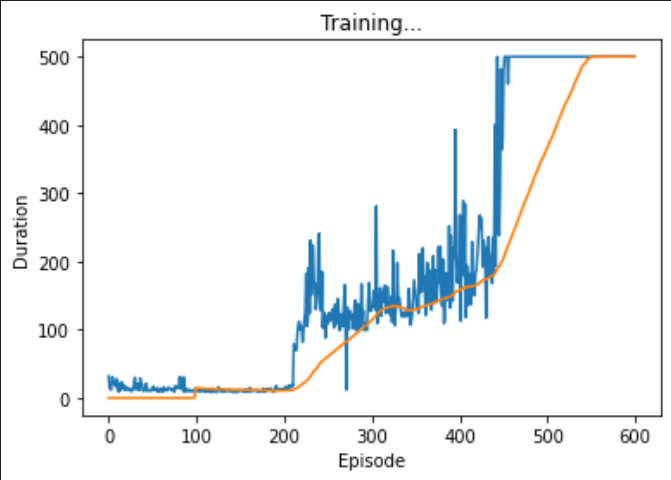
\includegraphics[width=\linewidth,cframe=blue 2.5pt 2.5pt]{agent600.png}
	\\	
	\vspace{0.1in}
	\textbf{Fig.3:} A trained agent with num\_episodes = 600
	\\
	\label{fig:Fig.3}
\end{figure}
\end{comment}













\end{document}